% =====================================================================
%  Measurement of Thermal Energy - Form Three Revision Notes
%  Print-ready A4 portrait, two-column student revision notes.
%  Build (run twice for TikZ/refs):
%    pdflatex -interaction=nonstopmode thermal-energy-notes.tex
% =====================================================================
\documentclass[10pt]{article}

% ---------- Encoding & fonts ----------
\usepackage[T1]{fontenc}
\usepackage[utf8]{inputenc}

% ---------- Page geometry: A4 portrait, tight margins ----------
\usepackage[a4paper,portrait,margin=1.2cm]{geometry}

% ---------- Maths ----------
\usepackage{amsmath}
\usepackage{amssymb}
\usepackage{siunitx}
\usepackage[version=4]{mhchem}

% ---------- Layout / boxes / graphics ----------
\usepackage{multicol}
\usepackage{tcolorbox}
\tcbuselibrary{skins,breakable}
\usepackage{xcolor}
\usepackage{enumitem}
\usepackage{graphicx}

% ---------- Keep section headings glued to the block that follows ----------
% Inside multicols a \section can land at a column/page boundary and get
% detached from the (unbreakable) definition box that follows it, leaving a
% blank column with the heading orphaned at its top and the body pushed to
% the next page (seen on page 1 with the "Heat Capacity" heading).
%
% Two coordinated measures fix this generally for every section:
%   1. needspace reserves vertical room *before* the heading, so a heading is
%      never emitted as the last line at the bottom of a column (see the
%      \section redefinition below).
%   2. LaTeX sets \@nobreaktrue after a heading, but that guard is only
%      honoured before a following *paragraph*; a tcolorbox's leading skip
%      ignores it. The \theme@boxbefore "before" code on the definition/nb/
%      example boxes restores the \nobreak for the box case, so a heading
%      cannot be split from a box that follows it (see the box definitions).
\usepackage{needspace}
\usepackage{etoolbox}
\makeatletter
% (1) Reserve space *before* every heading so a heading is never left dangling
%     as the last line at the bottom of a column.
\let\theme@oldsection\section
\renewcommand{\section}{%
  \needspace{8\baselineskip}%
  \theme@oldsection}
% (2) Standard LaTeX already sets \@nobreaktrue after a heading and, via
%     \everypar, forbids a break before the first *paragraph* that follows.
%     But when a tcolorbox (definition/nb/example) follows a heading directly,
%     its leading vertical skip is a raw \vskip that ignores \@nobreak, so
%     multicols may end the column right there and orphan the heading. The box
%     "before" code below (\if@nobreak\nobreak\fi) restores that guard for the
%     box case, so a heading stays glued to a following box just as it does to
%     following prose. This is general to every section.
\makeatother

% ---------- TikZ + libraries needed for later diagram work ----------
\usepackage{tikz}
\usetikzlibrary{arrows.meta,positioning,calc,decorations.pathmorphing}

% ---------------------------------------------------------------------
%  Colour palette
% ---------------------------------------------------------------------
\definecolor{defblue}{RGB}{31,97,141}
\definecolor{defbg}{RGB}{234,242,248}
\definecolor{nbred}{RGB}{176,58,46}
\definecolor{nbbg}{RGB}{250,235,233}
\definecolor{exgreen}{RGB}{30,110,80}
\definecolor{exbg}{RGB}{233,245,239}

% ---------------------------------------------------------------------
%  Reusable tcolorbox environments
% ---------------------------------------------------------------------
% "before" code keeps a box from breaking away from a preceding heading:
% \@afterheading sets \@nobreaktrue, so this inserts an infinite penalty
% before the box's leading skip in exactly that case (and does nothing
% otherwise, letting boxes break to the next column normally).
\makeatletter
\newcommand{\theme@boxbefore}{\par\if@nobreak\nobreak\fi\addvspace{5pt}\noindent}

% Definition box: coloured title bar reading "Definition"
\newtcolorbox{definition}[1][]{
  breakable,
  enhanced,
  colback=defbg,
  colframe=defblue,
  coltitle=white,
  fonttitle=\bfseries,
  title=Definition,
  boxrule=0.6pt,
  arc=2pt,
  left=4pt,right=4pt,top=3pt,bottom=3pt,
  before=\theme@boxbefore,
  #1
}

% NB call-out box: labelled "NB"
\newtcolorbox{nb}[1][]{
  breakable,
  enhanced,
  colback=nbbg,
  colframe=nbred,
  coltitle=white,
  fonttitle=\bfseries,
  title=NB,
  boxrule=0.6pt,
  arc=2pt,
  left=4pt,right=4pt,top=3pt,bottom=3pt,
  before=\theme@boxbefore,
  #1
}

% Worked-example box: optional title argument appended after "Worked Example"
\newtcolorbox{example}[1][]{
  breakable,
  enhanced,
  colback=exbg,
  colframe=exgreen,
  coltitle=white,
  fonttitle=\bfseries,
  title=Worked Example #1,
  boxrule=0.6pt,
  arc=2pt,
  left=4pt,right=4pt,top=3pt,bottom=3pt,
  before=\theme@boxbefore,
}
\makeatother

% ---------------------------------------------------------------------
%  Physics-solution layout helpers
%  Every worked example and numeric solution is laid out as
%  Given / Required / Formula / Working / Answer so the reader always
%  sees the data, the defined symbols, the governing equation and the
%  step-by-step algebra before the boxed result.
% ---------------------------------------------------------------------
\newcommand{\Given}{\par\vspace{2pt}\textbf{Given:}\ }
\newcommand{\Required}{\par\vspace{2pt}\textbf{Required:}\ }
\newcommand{\Formula}{\par\vspace{2pt}\textbf{Formula:}\ }
\newcommand{\Working}{\par\vspace{2pt}\textbf{Working:}}
\newcommand{\Answer}[1]{\par\vspace{2pt}\textbf{Answer:}\ \fbox{#1}}

% ---------------------------------------------------------------------
%  Document
% ---------------------------------------------------------------------
\setlength{\parindent}{0pt}
\setlength{\parskip}{4pt}
\pagestyle{plain}

\begin{document}

% ----- Title block (spans full page width) -----
\begin{center}
  {\LARGE\bfseries Measurement of Thermal Energy}\\[2pt]
  {\large Form Three Revision Notes}\\[4pt]
  \rule{\linewidth}{0.8pt}
\end{center}

\vspace{4pt}

% ----- Two-column body -----
\begin{multicols}{2}

% =====================================================================
\section{Temperature, Thermal Energy and the Kinetic Picture}
% =====================================================================
Every material is made of tiny particles (atoms or molecules) that are
always moving. In a solid they vibrate about fixed positions; in a
liquid they slide past one another; in a gas they fly about freely.
Because they move, the particles carry \emph{kinetic energy}, and
because they attract one another they also store \emph{potential
energy}. The total of all this microscopic energy is the internal
(thermal) energy of the body.

\begin{definition}
\textbf{Temperature} is a measure of the average kinetic energy of the
particles of a body. It tells us how hot or cold a body is, but not how
much heat energy the body contains. Its SI unit is the kelvin
(\si{\kelvin}); everyday work often uses degrees Celsius
(\si{\degreeCelsius}).
\end{definition}

\begin{definition}
\textbf{Thermal (internal) energy} is the total kinetic and potential
energy stored in all the particles of a body. It is a form of energy
and is measured in joules (\si{\joule}).
\end{definition}

\begin{nb}
Temperature and heat are not the same thing. A cup of boiling water is
hotter than a warm bath, yet the bath contains far more heat energy
because it has a much greater mass. Convert temperatures with
$T/\si{\kelvin} = \theta/\si{\degreeCelsius} + 273$. A \emph{change} of
temperature has the same size in \si{\kelvin} and \si{\degreeCelsius},
so $\Delta\theta$ may be quoted in either unit.
\end{nb}

\begin{nb}
\textbf{Symbols used in the worked solutions.}
$Q$ = heat energy (\si{\joule});
$m$ = mass (\si{\kilogram});
$c$ = specific heat capacity (\si{\joule\per\kilogram\per\kelvin});
$C$ = heat capacity (\si{\joule\per\kelvin});
$\Delta\theta$ = temperature change (\si{\kelvin});
$\theta$ = temperature (\si{\degreeCelsius});
$L_f$ = specific latent heat of fusion,
$L_v$ = specific latent heat of vapourisation (both \si{\joule\per\kilogram});
$P$ = power (\si{\watt}); $t$ = time (\si{\second}).
Each solution below sets out the \textbf{Given} data, the
\textbf{Required} unknown, the \textbf{Formula}, the step-by-step
\textbf{Working} and the final \textbf{Answer}.
\end{nb}

% =====================================================================
\section{Heat and What Determines It}
% =====================================================================
When two bodies at different temperatures are placed together, energy
flows from the hotter to the cooler one until they reach the same
temperature. That energy in transit is called heat.

\begin{definition}
\textbf{Heat} is the energy transferred from one body to another
because of a difference in temperature. Like all energy it is measured
in joules (\si{\joule}).
\end{definition}

The quantity of heat needed to warm a body depends on three things:
\begin{itemize}[leftmargin=*,nosep]
  \item the \textbf{mass} of the body (more mass needs more heat),
  \item the \textbf{temperature change} required (a bigger rise needs
        more heat),
  \item the \textbf{nature of the material} (different substances soak
        up heat differently).
\end{itemize}

% =====================================================================
\section{Heat Capacity}
% =====================================================================
\begin{definition}
\textbf{Heat capacity} $C$ of a body is the amount of heat energy
needed to raise the temperature of the \emph{whole body} by one kelvin
(or one degree Celsius):
\[
  C = \frac{Q}{\Delta\theta}, \qquad \text{unit: } \si{\joule\per\kelvin}.
\]
\end{definition}

\begin{nb}
Heat capacity refers to a particular object, so a large kettle of water
has a bigger heat capacity than a small cup of the same water. It does
not tell us anything about the material on its own.
\end{nb}

\begin{example}[: heat capacity of a block]
A heater delivers \SI{9600}{\joule} of energy to an iron block and its
temperature rises from \SI{20}{\degreeCelsius} to
\SI{60}{\degreeCelsius}. Find the heat capacity of the block.
\tcblower
\Given heat supplied $Q = \SI{9600}{\joule}$;
initial temperature $\theta_1 = \SI{20}{\degreeCelsius}$;
final temperature $\theta_2 = \SI{60}{\degreeCelsius}$.
\Required the heat capacity $C$ (\si{\joule\per\kelvin}).
\Formula $C = \dfrac{Q}{\Delta\theta}$, where
$\Delta\theta = \theta_2 - \theta_1$.
\Working
\begin{align*}
  \Delta\theta &= 60 - 20 = \SI{40}{\kelvin} \\
  C &= \frac{Q}{\Delta\theta} = \frac{\SI{9600}{\joule}}{\SI{40}{\kelvin}}
       = \SI{240}{\joule\per\kelvin}.
\end{align*}
\Answer{$C = \SI{240}{\joule\per\kelvin}$}
\end{example}

% =====================================================================
\section{Specific Heat Capacity}
% =====================================================================
\begin{definition}
\textbf{Specific heat capacity} $c$ of a substance is the amount of
heat energy needed to raise the temperature of \SI{1}{\kilogram} of the
substance by one kelvin:
\[
  c = \frac{Q}{m\,\Delta\theta}, \qquad
  \text{unit: } \si{\joule\per\kilogram\per\kelvin}.
\]
Rearranging gives the heat equation used constantly in this topic:
\[
  \boxed{\,Q = m\,c\,\Delta\theta\,}
\]
\end{definition}

\begin{nb}
Water has an unusually large specific heat capacity
($\SI{4200}{\joule\per\kilogram\per\kelvin}$). This is why water heats
up slowly, cools down slowly and is used as a coolant in car engines
and as a store of heat in hot-water systems.
\end{nb}

\begin{center}
\small
\begin{tabular}{@{}lc@{}}
\multicolumn{2}{c}{\textbf{Typical specific heat capacities}}\\[2pt]
\hline
Substance & $c$ (\si{\joule\per\kilogram\per\kelvin}) \\
\hline
Water        & 4200 \\
Ice          & 2100 \\
Steam        & 2010 \\
Aluminium    & 900  \\
Iron         & 480  \\
Copper       & 390  \\
Brass        & 320  \\
Lead         & 130  \\
\hline
\end{tabular}
\end{center}

\begin{example}[: warming water]
How much heat is needed to raise the temperature of \SI{2.5}{\kilogram}
of water from \SI{20}{\degreeCelsius} to \SI{80}{\degreeCelsius}?
Take $c_{\text{water}} = \SI{4200}{\joule\per\kilogram\per\kelvin}$.
\tcblower
\Given mass $m = \SI{2.5}{\kilogram}$;
specific heat capacity $c = \SI{4200}{\joule\per\kilogram\per\kelvin}$;
$\theta_1 = \SI{20}{\degreeCelsius}$, $\theta_2 = \SI{80}{\degreeCelsius}$.
\Required the heat supplied $Q$ (\si{\joule}).
\Formula $Q = m\,c\,\Delta\theta$, with $\Delta\theta = \theta_2 - \theta_1$.
\Working
\begin{align*}
  \Delta\theta &= 80 - 20 = \SI{60}{\kelvin} \\
  Q &= m\,c\,\Delta\theta \\
    &= 2.5 \times 4200 \times 60 \\
    &= \SI{630000}{\joule} = \SI{630}{\kilo\joule}.
\end{align*}
\Answer{$Q = \SI{630}{\kilo\joule}$}
\end{example}

\begin{example}[: heating a metal block]
An aluminium block of mass \SI{0.8}{\kilogram} is heated from
\SI{25}{\degreeCelsius} to \SI{175}{\degreeCelsius}. Find the heat
supplied. Take $c_{\text{Al}} =
\SI{900}{\joule\per\kilogram\per\kelvin}$.
\tcblower
\Given mass $m = \SI{0.8}{\kilogram}$;
$c = \SI{900}{\joule\per\kilogram\per\kelvin}$;
$\theta_1 = \SI{25}{\degreeCelsius}$, $\theta_2 = \SI{175}{\degreeCelsius}$.
\Required the heat supplied $Q$ (\si{\joule}).
\Formula $Q = m\,c\,\Delta\theta$, with $\Delta\theta = \theta_2 - \theta_1$.
\Working
\begin{align*}
  \Delta\theta &= 175 - 25 = \SI{150}{\kelvin} \\
  Q &= m\,c\,\Delta\theta = 0.8 \times 900 \times 150 \\
    &= \SI{108000}{\joule} = \SI{108}{\kilo\joule}.
\end{align*}
\Answer{$Q = \SI{108}{\kilo\joule}$}
\end{example}

\begin{example}[: finding specific heat capacity]
A \SI{0.5}{\kilogram} copper cylinder is given \SI{7800}{\joule} of
heat and its temperature rises by \SI{40}{\kelvin}. Find its specific
heat capacity.
\tcblower
\Given mass $m = \SI{0.5}{\kilogram}$;
heat supplied $Q = \SI{7800}{\joule}$;
temperature change $\Delta\theta = \SI{40}{\kelvin}$.
\Required the specific heat capacity $c$
(\si{\joule\per\kilogram\per\kelvin}).
\Formula $Q = m\,c\,\Delta\theta \Rightarrow c = \dfrac{Q}{m\,\Delta\theta}$.
\Working
\begin{align*}
  c &= \frac{Q}{m\,\Delta\theta}
     = \frac{7800}{0.5 \times 40} \\
    &= \frac{7800}{20}
     = \SI{390}{\joule\per\kilogram\per\kelvin}.
\end{align*}
This matches the value for copper in the table above.
\Answer{$c = \SI{390}{\joule\per\kilogram\per\kelvin}$}
\end{example}

% =====================================================================
\section{Calorimetry and the Method of Mixtures}
% =====================================================================
A \textbf{calorimeter} is a well-lagged metal container used to measure
quantities of heat. When a hot body is placed with a cold one inside
it, they exchange heat until they settle at a common
(\emph{equilibrium}) temperature.

\begin{center}
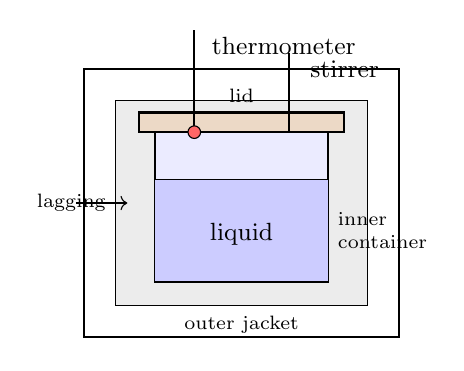
\begin{tikzpicture}[scale=1.0,every node/.style={font=\small}]
  % outer jacket
  \draw[thick] (0,0) rectangle (4,3.4);
  % lagging (hatched gap)
  \draw[fill=gray!15] (0.4,0.4) rectangle (3.6,3.0);
  \node at (2,0.15) {\scriptsize outer jacket};
  % inner container
  \draw[thick,fill=blue!8] (0.9,0.7) rectangle (3.1,2.6);
  % liquid
  \draw[fill=blue!20] (0.9,0.7) rectangle (3.1,2.0);
  \node at (2.0,1.3) {liquid};
  % lid
  \draw[thick,fill=brown!30] (0.7,2.6) rectangle (3.3,2.85);
  % thermometer
  \draw[thick] (1.4,2.6) -- (1.4,3.9);
  \draw[fill=red!60] (1.4,2.6) circle (0.08);
  \node[right] at (1.5,3.7) {thermometer};
  % stirrer
  \draw[thick] (2.6,2.6) -- (2.6,3.6);
  \draw[thick] (2.45,2.6) -- (2.75,2.6);
  \node[right] at (2.75,3.4) {stirrer};
  % labels
  \node[left] at (0.4,1.7) {\scriptsize lagging};
  \draw[->] (-0.1,1.7) -- (0.55,1.7);
  \node[right] at (3.1,1.5) {\scriptsize inner};
  \node[right] at (3.1,1.2) {\scriptsize container};
  \node[above] at (2,2.85) {\scriptsize lid};
\end{tikzpicture}\\[-2pt]
{\scriptsize\textbf{Fig.\ 1} A lagged calorimeter used in
mixtures experiments. \textit{(See the corresponding figure in your
textbook's chapter on thermal energy.)}}
\end{center}

\begin{definition}
\textbf{The principle of mixtures} (conservation of energy): if no heat
escapes to the surroundings, the heat lost by the hot body equals the
heat gained by the cold body:
\[
  \boxed{\;Q_{\text{lost}} = Q_{\text{gained}}\;}
\]
\end{definition}

\begin{nb}
The container (calorimeter) and stirrer also absorb heat. In careful
work their heat capacity is included. In these notes we assume a
perfectly lagged calorimeter of negligible heat capacity unless stated
otherwise.
\end{nb}

\begin{example}[: equilibrium temperature]
\SI{0.3}{\kilogram} of water at \SI{80}{\degreeCelsius} is mixed with
\SI{0.5}{\kilogram} of water at \SI{20}{\degreeCelsius}. Find the final
temperature $\theta$.
\tcblower
\Given hot water $m_1 = \SI{0.3}{\kilogram}$ at
$\theta_1 = \SI{80}{\degreeCelsius}$;
cold water $m_2 = \SI{0.5}{\kilogram}$ at
$\theta_2 = \SI{20}{\degreeCelsius}$; same liquid, so $c$ is common.
\Required the equilibrium temperature $\theta$ (\si{\degreeCelsius}).
\Formula principle of mixtures: $Q_{\text{lost}} = Q_{\text{gained}}$,
i.e. $m_1 c(\theta_1 - \theta) = m_2 c(\theta - \theta_2)$ ($c$ cancels).
\Working
\begin{align*}
  m_1 c (80 - \theta) &= m_2 c (\theta - 20) \\
  0.3(80 - \theta) &= 0.5(\theta - 20) \\
  24 - 0.3\theta &= 0.5\theta - 10 \\
  34 &= 0.8\theta \\
  \theta &= \SI{42.5}{\degreeCelsius}.
\end{align*}
\Answer{$\theta = \SI{42.5}{\degreeCelsius}$}
\end{example}

\begin{example}[: specific heat capacity of a metal]
A \SI{0.4}{\kilogram} metal block heated to \SI{100}{\degreeCelsius} is
dropped into \SI{0.2}{\kilogram} of water at \SI{18}{\degreeCelsius} in
a calorimeter of negligible heat capacity. The mixture settles at
\SI{30}{\degreeCelsius}. Find the specific heat capacity $c_m$ of the
metal.
\tcblower
\Given metal $m_m = \SI{0.4}{\kilogram}$ at
\SI{100}{\degreeCelsius}; water $m_w = \SI{0.2}{\kilogram}$,
$c_w = \SI{4200}{\joule\per\kilogram\per\kelvin}$ at
\SI{18}{\degreeCelsius}; equilibrium $\theta = \SI{30}{\degreeCelsius}$.
\Required the specific heat capacity $c_m$ of the metal.
\Formula $Q_{\text{lost by metal}} = Q_{\text{gained by water}}$, i.e.
$m_m c_m(100 - \theta) = m_w c_w(\theta - 18)$.
\Working
\begin{align*}
  m_m c_m (100 - 30) &= m_w c_w (30 - 18) \\
  0.4 \, c_m \times 70 &= 0.2 \times 4200 \times 12 \\
  28\,c_m &= 10080 \\
  c_m &= \SI{360}{\joule\per\kilogram\per\kelvin}.
\end{align*}
\Answer{$c_m = \SI{360}{\joule\per\kilogram\per\kelvin}$}
\end{example}

\begin{example}[: finding an unknown mass]
An unknown mass $m$ of water at \SI{15}{\degreeCelsius} is added to
\SI{0.6}{\kilogram} of water at \SI{75}{\degreeCelsius}. The mixture
reaches \SI{55}{\degreeCelsius}. Find $m$ (ignore the container).
\tcblower
\Given cold water mass $m$ (unknown) at \SI{15}{\degreeCelsius};
hot water $m_2 = \SI{0.6}{\kilogram}$ at \SI{75}{\degreeCelsius};
equilibrium $\theta = \SI{55}{\degreeCelsius}$; common $c$ (water).
\Required the unknown mass $m$ (\si{\kilogram}).
\Formula $Q_{\text{gained by cold}} = Q_{\text{lost by hot}}$, i.e.
$m\,c(\theta - 15) = m_2 c(75 - \theta)$ ($c$ cancels).
\Working
\begin{align*}
  m\,c(55 - 15) &= 0.6\,c(75 - 55) \\
  40\,m &= 0.6 \times 20 \\
  40\,m &= 12 \\
  m &= \SI{0.3}{\kilogram}.
\end{align*}
\Answer{$m = \SI{0.3}{\kilogram}$}
\end{example}

\begin{example}[: specific heat capacity of a liquid]
A heater rated \SI{50}{\watt} warms \SI{0.25}{\kilogram} of an oil by
\SI{16}{\kelvin} in \SI{2}{\minute}. Assuming no losses, find the
specific heat capacity of the oil.
\tcblower
\Given power $P = \SI{50}{\watt}$; mass $m = \SI{0.25}{\kilogram}$;
temperature change $\Delta\theta = \SI{16}{\kelvin}$;
time $t = \SI{2}{\minute} = \SI{120}{\second}$.
\Required the specific heat capacity $c$ of the oil.
\Formula heat delivered $Q = P\,t$, then
$c = \dfrac{Q}{m\,\Delta\theta}$.
\Working
\begin{align*}
  Q &= P\,t = 50 \times (2 \times 60) = \SI{6000}{\joule} \\
  c &= \frac{Q}{m\,\Delta\theta} = \frac{6000}{0.25 \times 16} \\
    &= \frac{6000}{4} = \SI{1500}{\joule\per\kilogram\per\kelvin}.
\end{align*}
\Answer{$c = \SI{1500}{\joule\per\kilogram\per\kelvin}$}
\end{example}

% =====================================================================
\section{Change of State and the Kinetic Theory}
% =====================================================================
Matter exists in three common states: solid, liquid and gas. Adding or
removing heat can change one state into another. The kinetic theory
explains this by how strongly the particles are held together and how
fast they move.

\begin{center}
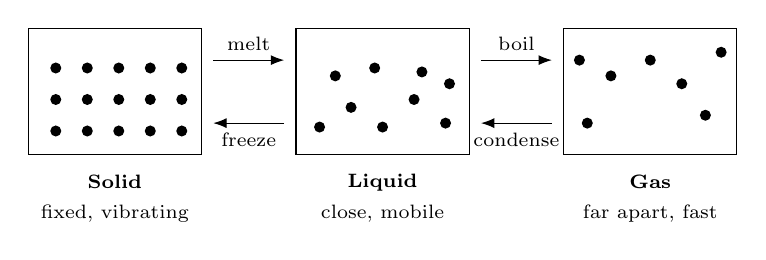
\begin{tikzpicture}[scale=1.0,every node/.style={font=\scriptsize}]
  % solid
  \draw (0,0) rectangle (2.2,1.6);
  \foreach \x in {0.35,0.75,1.15,1.55,1.95}
    \foreach \y in {0.3,0.7,1.1}
      \fill (\x,\y) circle (0.07);
  \node at (1.1,-0.35) {\textbf{Solid}};
  \node at (1.1,-0.75) {fixed, vibrating};
  % liquid
  \draw (3.4,0) rectangle (5.6,1.6);
  \foreach \p in {(3.7,0.35),(4.1,0.6),(4.5,0.35),(4.9,0.7),(5.3,0.4),
                  (3.9,1.0),(4.4,1.1),(5.0,1.05),(5.35,0.9)}
    \fill \p circle (0.07);
  \node at (4.5,-0.35) {\textbf{Liquid}};
  \node at (4.5,-0.75) {close, mobile};
  % gas
  \draw (6.8,0) rectangle (9.0,1.6);
  \foreach \p in {(7.1,0.4),(7.9,1.2),(8.6,0.5),(7.4,1.0),(8.3,0.9),
                  (8.8,1.3),(7.0,1.2)}
    \fill \p circle (0.07);
  \node at (7.9,-0.35) {\textbf{Gas}};
  \node at (7.9,-0.75) {far apart, fast};
  % arrows
  \draw[-{Latex}] (2.35,1.2) -- (3.25,1.2) node[midway,above]{melt};
  \draw[-{Latex}] (3.25,0.4) -- (2.35,0.4) node[midway,below]{freeze};
  \draw[-{Latex}] (5.75,1.2) -- (6.65,1.2) node[midway,above]{boil};
  \draw[-{Latex}] (6.65,0.4) -- (5.75,0.4) node[midway,below]{condense};
\end{tikzpicture}\\[8pt]
{\scriptsize\textbf{Fig.\ 2} The three states of water and the changes
between them. \textit{(See the corresponding figure in your textbook.)}}
\end{center}

\begin{definition}
\textbf{Melting} is the change from solid to liquid at a fixed
temperature called the \textbf{melting point}. \textbf{Freezing} is the
reverse change from liquid to solid at the same temperature (the
\textbf{freezing point}). For a pure substance the two are equal.
\end{definition}

\begin{nb}
While a pure solid melts, the temperature stays constant even though
heat is still being supplied. The energy goes into breaking the bonds
between particles, not into raising their speed.
\end{nb}

\begin{center}
\begin{tikzpicture}[scale=1.0,every node/.style={font=\scriptsize}]
  \draw[-{Latex}] (0,0) -- (6.6,0) node[right]{time};
  \draw[-{Latex}] (0,0) -- (0,3.4) node[above]{temperature};
  % cooling: liquid falls, plateau (freezing), then solid falls
  \draw[thick,blue] (0.3,3.1) .. controls (1.2,2.3) .. (2.0,2.0)
        -- (4.0,2.0)
        .. controls (5.0,1.6) .. (6.2,0.7);
  \draw[dashed] (0,2.0) -- (2.0,2.0);
  \node[left] at (0,2.0) {$\theta_f$};
  \node at (3.0,2.25) {freezing plateau};
  \node at (1.0,2.9) {liquid};
  \node at (5.3,1.4) {solid};
\end{tikzpicture}\\[2pt]
{\scriptsize\textbf{Fig.\ 3} Cooling curve: a liquid cooling to a solid
shows a flat plateau at the freezing point $\theta_f$.
\textit{(See the corresponding figure in your textbook.)}}
\end{center}

\begin{example}[: cooling through the freezing point]
A pure substance of mass \SI{0.2}{\kilogram} is liquid at
\SI{90}{\degreeCelsius} and freezes at \SI{60}{\degreeCelsius}. Its
specific heat capacity as a liquid is
\SI{2500}{\joule\per\kilogram\per\kelvin} and its specific latent heat
of fusion is \SI{80000}{\joule\per\kilogram}. Find the total heat
removed to cool the liquid to \SI{60}{\degreeCelsius} and then freeze it
completely.
\tcblower
\Given mass $m = \SI{0.2}{\kilogram}$; liquid at
\SI{90}{\degreeCelsius}; freezing point \SI{60}{\degreeCelsius};
$c = \SI{2500}{\joule\per\kilogram\per\kelvin}$;
$L_f = \SI{80000}{\joule\per\kilogram}$.
\Required the total heat removed $Q_{\text{total}}$ (\si{\joule}).
\Formula cool the liquid with $Q_1 = m c\,\Delta\theta$, then freeze it
with $Q_2 = m L_f$; total $Q_{\text{total}} = Q_1 + Q_2$.
\Working
\begin{align*}
  Q_1 &= m c \,\Delta\theta = 0.2 \times 2500 \times (90 - 60) \\
      &= \SI{15000}{\joule} \\
  Q_2 &= m L_f = 0.2 \times 80000 = \SI{16000}{\joule} \\
  Q_{\text{total}} &= Q_1 + Q_2 = \SI{31000}{\joule} = \SI{31}{\kilo\joule}.
\end{align*}
\Answer{$Q_{\text{total}} = \SI{31}{\kilo\joule}$}
\end{example}

% =====================================================================
\section{Effect of Impurities and Pressure; Regelation}
% =====================================================================
\begin{itemize}[leftmargin=*,nosep]
  \item \textbf{Impurities} lower the melting/freezing point. Salt
        spread on icy roads makes the ice melt below
        \SI{0}{\degreeCelsius}.
  \item \textbf{Increasing pressure lowers} the melting point of ice
        (ice is unusual because it expands on freezing). For most
        substances higher pressure raises the melting point.
\end{itemize}

\begin{definition}
\textbf{Regelation} is the melting of ice under pressure and its
re-freezing once the pressure is removed. A thin wire loaded with
weights slowly passes through a block of ice while the block stays in
one piece behind it.
\end{definition}

\begin{center}
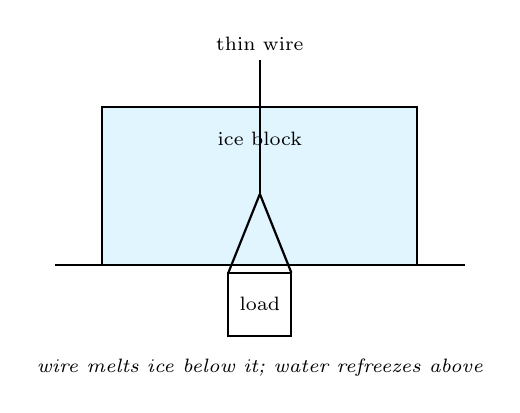
\begin{tikzpicture}[scale=1.0,every node/.style={font=\scriptsize}]
  % ice block
  \draw[thick,fill=cyan!12] (0,0) rectangle (4,2);
  \node at (2,1.6) {ice block};
  % wire over the top
  \draw[thick] (2,2.6) -- (2,0.9);
  \node[above] at (2,2.6) {thin wire};
  % weights
  \draw[thick] (1.6,-0.9) rectangle (2.4,-0.1);
  \draw[thick] (2,0.9) -- (1.6,-0.1);
  \draw[thick] (2,0.9) -- (2.4,-0.1);
  \node at (2,-0.5) {load};
  % supports
  \draw[thick] (-0.6,0) -- (4.6,0);
  \node at (2,-1.3) {\itshape wire melts ice below it; water refreezes above};
\end{tikzpicture}\\[2pt]
{\scriptsize\textbf{Fig.\ 4} Regelation: a loaded wire cuts through
ice which re-freezes behind it.
\textit{(See the corresponding figure in your textbook.)}}
\end{center}

% =====================================================================
\section{Boiling and Evaporation}
% =====================================================================
Both boiling and evaporation turn a liquid into a gas, but they are not
the same process.

\begin{definition}
\textbf{Boiling} is the rapid change of a liquid to vapour throughout
the whole liquid at a fixed temperature, the \textbf{boiling point}.
\textbf{Evaporation} is the slow escape of the fastest molecules from
the surface of a liquid, and it happens at all temperatures.
\end{definition}

\begin{center}
\small
\begin{tabular}{@{}p{3.2cm}p{3.2cm}@{}}
\hline
\textbf{Boiling} & \textbf{Evaporation} \\
\hline
Occurs at a fixed temperature & Occurs at any temperature \\
Throughout the liquid & Only at the surface \\
Bubbles form in the bulk & No bubbles \\
Needs continuous heating & Can occur without added heat \\
\hline
\end{tabular}
\end{center}

The boiling point is affected by:
\begin{itemize}[leftmargin=*,nosep]
  \item \textbf{Impurities:} dissolved substances raise the boiling
        point (salty water boils above \SI{100}{\degreeCelsius}).
  \item \textbf{Pressure:} higher pressure raises the boiling point
        (a pressure cooker cooks faster). Lower pressure lowers it.
  \item \textbf{Altitude:} on high mountains the air pressure is low,
        so water boils below \SI{100}{\degreeCelsius}.
\end{itemize}

\begin{center}
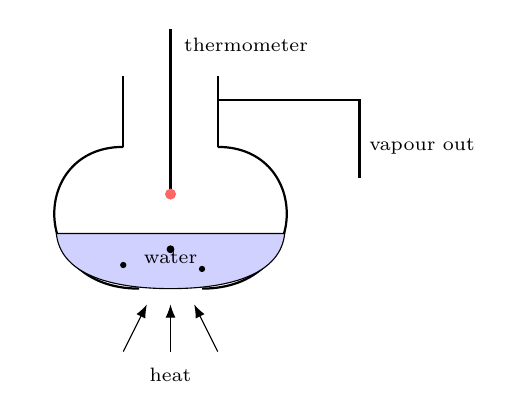
\begin{tikzpicture}[scale=1.0,every node/.style={font=\scriptsize}]
  % round-bottomed flask
  \draw[thick] (1.6,0.2) .. controls (0.2,0.2) and (0.2,2.0) .. (1.4,2.0);
  \draw[thick] (2.4,0.2) .. controls (3.8,0.2) and (3.8,2.0) .. (2.6,2.0);
  \draw[thick] (1.4,2.0) -- (1.4,2.9);
  \draw[thick] (2.6,2.0) -- (2.6,2.9);
  % liquid
  \draw[fill=blue!18] (0.55,0.9) .. controls (0.6,0.4) and (1.2,0.2) ..
        (2.0,0.2) .. controls (2.8,0.2) and (3.4,0.4) .. (3.45,0.9)
        -- cycle;
  \node at (2.0,0.6) {water};
  % bubbles
  \fill (1.4,0.5) circle (0.04); \fill (2.4,0.45) circle (0.04);
  \fill (2.0,0.7) circle (0.05);
  % thermometer
  \draw[thick] (2.0,1.4) -- (2.0,3.5);
  \fill[red!60] (2.0,1.4) circle (0.07);
  \node[right] at (2.05,3.3) {thermometer};
  % delivery tube
  \draw[thick] (2.6,2.6) -- (4.4,2.6) -- (4.4,1.6);
  \node[right] at (4.4,2.0) {vapour out};
  % heat
  \draw[-{Latex}] (1.4,-0.6) -- (1.7,0.0);
  \draw[-{Latex}] (2.0,-0.6) -- (2.0,0.0);
  \draw[-{Latex}] (2.6,-0.6) -- (2.3,0.0);
  \node at (2.0,-0.9) {heat};
\end{tikzpicture}\\[2pt]
{\scriptsize\textbf{Fig.\ 5} Boiling apparatus for observing the
boiling point. \textit{(See the corresponding figure in your textbook.)}}
\end{center}

\begin{center}
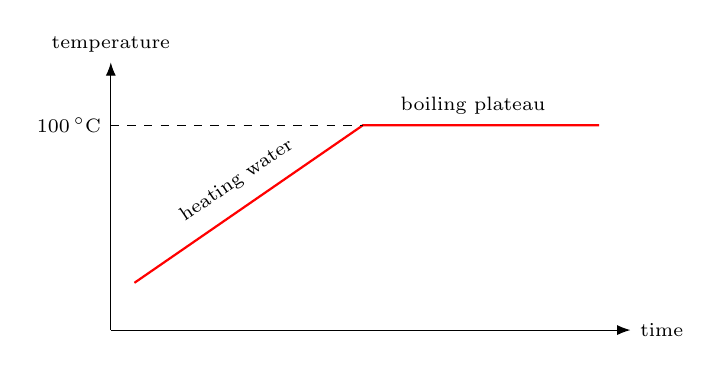
\begin{tikzpicture}[scale=1.0,every node/.style={font=\scriptsize}]
  \draw[-{Latex}] (0,0) -- (6.6,0) node[right]{time};
  \draw[-{Latex}] (0,0) -- (0,3.4) node[above]{temperature};
  \draw[thick,red] (0.3,0.6) -- (3.2,2.6) -- (6.2,2.6);
  \draw[dashed] (0,2.6) -- (3.2,2.6);
  \node[left] at (0,2.6) {\SI{100}{\celsius}};
  \node at (4.6,2.85) {boiling plateau};
  \node[rotate=34] at (1.6,1.9) {heating water};
\end{tikzpicture}\\[2pt]
{\scriptsize\textbf{Fig.\ 6} Heating water: the temperature rises then
stays flat while the water boils.
\textit{(See the corresponding figure in your textbook.)}}
\end{center}

% =====================================================================
\section{Latent Heat}
% =====================================================================
During a change of state heat is absorbed or released with \emph{no
change in temperature}. This ``hidden'' heat is called latent heat.

\begin{definition}
\textbf{Specific latent heat of fusion} $L_f$ is the heat needed to
change \SI{1}{\kilogram} of a solid into liquid at its melting point
without a change in temperature.
\textbf{Specific latent heat of vapourisation} $L_v$ is the heat needed
to change \SI{1}{\kilogram} of a liquid into vapour at its boiling
point. In both cases:
\[
  \boxed{\,Q = m\,L\,}, \qquad \text{unit of } L:\ \si{\joule\per\kilogram}.
\]
\end{definition}

\begin{nb}
For water: $L_f = \SI{3.34e5}{\joule\per\kilogram}$ and
$L_v = \SI{2.26e6}{\joule\per\kilogram}$. Vapourisation absorbs far more
energy than fusion, which is why steam at \SI{100}{\degreeCelsius}
causes worse scalds than the same mass of boiling water.
\end{nb}

\begin{center}
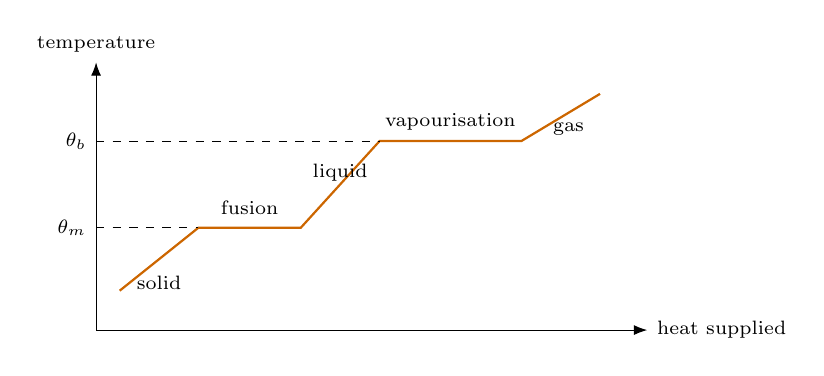
\begin{tikzpicture}[scale=1.0,every node/.style={font=\scriptsize}]
  \draw[-{Latex}] (0,0) -- (7.0,0) node[right]{heat supplied};
  \draw[-{Latex}] (0,0) -- (0,3.4) node[above]{temperature};
  \draw[thick,orange!80!black]
        (0.3,0.5) -- (1.3,1.3)   % solid warming
        -- (2.6,1.3)             % fusion plateau
        -- (3.6,2.4)             % liquid warming
        -- (5.4,2.4)             % vapourisation plateau
        -- (6.4,3.0);            % gas warming
  \draw[dashed] (0,1.3) -- (1.3,1.3); \node[left] at (0,1.3){$\theta_m$};
  \draw[dashed] (0,2.4) -- (3.6,2.4); \node[left] at (0,2.4){$\theta_b$};
  \node at (0.8,0.6) {solid};
  \node at (1.95,1.55) {fusion};
  \node at (3.1,2.0) {liquid};
  \node at (4.5,2.65) {vapourisation};
  \node at (6.0,2.55) {gas};
\end{tikzpicture}\\[2pt]
{\scriptsize\textbf{Fig.\ 7} Temperature versus heat supplied: two flat
plateaus mark fusion and vapourisation.
\textit{(See the corresponding figure in your textbook.)}}
\end{center}

\begin{example}[: melting ice]
Find the heat needed to melt \SI{0.4}{\kilogram} of ice already at
\SI{0}{\degreeCelsius}. Take
$L_f = \SI{3.34e5}{\joule\per\kilogram}$.
\tcblower
\Given mass $m = \SI{0.4}{\kilogram}$ of ice at
\SI{0}{\degreeCelsius}; $L_f = \SI{3.34e5}{\joule\per\kilogram}$.
\Required the heat $Q$ needed to melt it (\si{\joule}).
\Formula at the melting point (no temperature change) $Q = m L_f$.
\Working
\begin{align*}
  Q &= m L_f = 0.4 \times 3.34\times10^{5} \\
    &= \SI{133600}{\joule} \approx \SI{134}{\kilo\joule}.
\end{align*}
\Answer{$Q \approx \SI{134}{\kilo\joule}$}
\end{example}

\begin{example}[: ice to steam in stages]
Find the total heat to change \SI{0.1}{\kilogram} of ice at
\SI{-10}{\degreeCelsius} into steam at \SI{120}{\degreeCelsius}. Use
$c_{\text{ice}}=2100$, $c_{\text{water}}=4200$, $c_{\text{steam}}=2010$
(\si{\joule\per\kilogram\per\kelvin}),
$L_f=\SI{3.34e5}{\joule\per\kilogram}$,
$L_v=\SI{2.26e6}{\joule\per\kilogram}$.
\tcblower
\Given mass $m = \SI{0.1}{\kilogram}$;
$c_{\text{ice}}=2100$, $c_{\text{water}}=4200$, $c_{\text{steam}}=2010$
(\si{\joule\per\kilogram\per\kelvin});
$L_f=\SI{3.34e5}{\joule\per\kilogram}$,
$L_v=\SI{2.26e6}{\joule\per\kilogram}$; ice at
\SI{-10}{\degreeCelsius} to steam at \SI{120}{\degreeCelsius}.
\Required the total heat $Q_{\text{tot}}$ (\si{\joule}).
\Formula five stages: warm ice ($Q_1=mc_{\text{ice}}\Delta\theta$),
melt ($Q_2=mL_f$), warm water ($Q_3=mc_{\text{w}}\Delta\theta$),
boil ($Q_4=mL_v$), warm steam ($Q_5=mc_{\text{st}}\Delta\theta$);
$Q_{\text{tot}}=Q_1+Q_2+Q_3+Q_4+Q_5$.
\Working
\begin{align*}
  Q_1 &= m c_{\text{ice}}\,\Delta\theta = 0.1\times2100\times10 = \SI{2100}{\joule}\\
  Q_2 &= m L_f = 0.1\times3.34\times10^{5} = \SI{33400}{\joule}\\
  Q_3 &= m c_{\text{w}}\,\Delta\theta = 0.1\times4200\times100 = \SI{42000}{\joule}\\
  Q_4 &= m L_v = 0.1\times2.26\times10^{6} = \SI{226000}{\joule}\\
  Q_5 &= m c_{\text{st}}\,\Delta\theta = 0.1\times2010\times20 = \SI{4020}{\joule}\\
  Q_{\text{tot}} &= Q_1+Q_2+Q_3+Q_4+Q_5\\
      &= \SI{307520}{\joule} \approx \SI{308}{\kilo\joule}.
\end{align*}
\Answer{$Q_{\text{tot}} \approx \SI{308}{\kilo\joule}$}
\end{example}

\begin{center}
\begin{tikzpicture}[scale=1.0,every node/.style={font=\scriptsize}]
  \draw[-{Latex}] (0,0) -- (7.0,0) node[right]{heat supplied};
  \draw[-{Latex}] (0,0) -- (0,3.4) node[above]{temperature (\si{\celsius})};
  \draw[thick,blue]
        (0.3,0.5) -- (0.9,0.9)   % ice -10 to 0
        -- (2.0,0.9)             % melting plateau
        -- (3.0,2.3)             % water 0 to 100
        -- (5.4,2.3)             % boiling plateau
        -- (6.2,2.9);            % steam 100 to 120
  \draw[dashed] (0,0.9) -- (0.9,0.9); \node[left] at (0,0.9){$0$};
  \draw[dashed] (0,2.3) -- (3.0,2.3); \node[left] at (0,2.3){$100$};
  \node at (0.55,0.45) {ice};
  \node at (1.45,1.15) {melting};
  \node at (2.5,1.8) {water};
  \node at (4.2,2.55) {boiling};
  \node at (5.9,2.45) {steam};
\end{tikzpicture}\\[2pt]
{\scriptsize\textbf{Fig.\ 8} Staged heating of ice at
\SI{-10}{\celsius} to steam at \SI{120}{\celsius}.
\textit{(See the corresponding figure in your textbook.)}}
\end{center}

\begin{example}[: steam condensing to warm water]
Steam at \SI{100}{\degreeCelsius} is passed into \SI{0.5}{\kilogram} of
water at \SI{20}{\degreeCelsius} until the water reaches
\SI{40}{\degreeCelsius}. The condensed steam then cools from
\SI{100}{\degreeCelsius} to \SI{40}{\degreeCelsius}. Find the mass $m_s$
of steam condensed. Use
$L_v=\SI{2.26e6}{\joule\per\kilogram}$, $c_w=4200$.
\tcblower
\Given cold water $m_w = \SI{0.5}{\kilogram}$ warmed from
\SI{20}{} to \SI{40}{\degreeCelsius}; steam mass $m_s$ (unknown)
condensing at \SI{100}{\degreeCelsius} then cooling to
\SI{40}{\degreeCelsius}; $L_v=\SI{2.26e6}{\joule\per\kilogram}$,
$c_w=\SI{4200}{\joule\per\kilogram\per\kelvin}$.
\Required the mass of steam condensed $m_s$ (\si{\kilogram}).
\Formula heat released by steam $=$ heat gained by cold water:
$m_s L_v + m_s c_w(100-40) = m_w c_w(40-20)$.
\Working
\begin{align*}
  m_s L_v + m_s c_w(100-40) &= m_w c_w(40-20) \\
  m_s(2.26\times10^{6} + 4200\times60) &= 0.5\times4200\times20 \\
  m_s(2.26\times10^{6} + 2.52\times10^{5}) &= 42000 \\
  m_s \times 2.512\times10^{6} &= 42000 \\
  m_s &\approx \SI{0.0167}{\kilogram} = \SI{16.7}{\gram}.
\end{align*}
\Answer{$m_s \approx \SI{16.7}{\gram}$}
\end{example}

\begin{example}[: energy and time to melt lead]
A heater rated \SI{300}{\watt} melts \SI{0.5}{\kilogram} of lead already
at its melting point. Take $L_f(\text{lead}) =
\SI{25000}{\joule\per\kilogram}$. Find the energy required and the time
taken, assuming no heat is lost.
\tcblower
\Given power $P = \SI{300}{\watt}$; mass $m = \SI{0.5}{\kilogram}$ at
the melting point; $L_f = \SI{25000}{\joule\per\kilogram}$.
\Required the energy $Q$ (\si{\joule}) and the time $t$ (\si{\second}).
\Formula $Q = m L_f$, then $t = \dfrac{Q}{P}$.
\Working
\begin{align*}
  Q &= m L_f = 0.5 \times 25000 = \SI{12500}{\joule} \\
  t &= \frac{Q}{P} = \frac{12500}{300} \approx \SI{41.7}{\second}.
\end{align*}
\Answer{$Q = \SI{12.5}{\kilo\joule}$, $t \approx \SI{41.7}{\second}$}
\end{example}

% =====================================================================
\section{Cooling by Evaporation and the Refrigerator}
% =====================================================================
When a liquid evaporates, the fastest molecules escape, so the average
kinetic energy of those left behind falls. This is why evaporation
cools: sweat drying on the skin, or a wet cloth round a water pot, both
feel cold. Volatile liquids (methylated spirit, ether) evaporate fast
and produce strong cooling.

\begin{definition}
A \textbf{refrigerator} uses a volatile working fluid (refrigerant)
that evaporates inside the freezer coils, taking latent heat from the
food, and then condenses in the coils behind the fridge, giving that
heat out to the room.
\end{definition}

\begin{center}
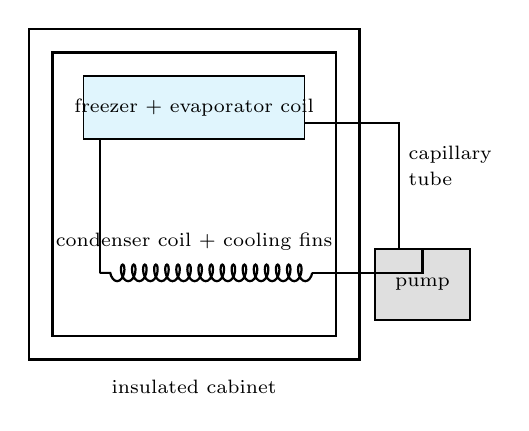
\begin{tikzpicture}[scale=1.0,every node/.style={font=\scriptsize}]
  % cabinet double wall
  \draw[thick] (0,0) rectangle (4.2,4.2);
  \draw[thick] (0.3,0.3) rectangle (3.9,3.9);
  \node at (2.1,-0.35) {insulated cabinet};
  % freezing compartment with evaporator coil
  \draw[fill=cyan!12] (0.7,2.8) rectangle (3.5,3.6);
  \node at (2.1,3.2) {freezer + evaporator coil};
  % capillary tube
  \draw[thick] (3.5,3.0) -- (4.7,3.0) -- (4.7,1.4);
  \node[right] at (4.7,2.6) {capillary};
  \node[right] at (4.7,2.3) {tube};
  % compressor pump
  \draw[thick,fill=gray!25] (4.4,0.5) rectangle (5.6,1.4);
  \node at (5.0,0.95) {pump};
  % condenser + fins behind
  \draw[thick] (4.4,1.1) -- (3.6,1.1);
  \draw[thick,decorate,decoration={coil,segment length=4pt,amplitude=3pt}]
       (3.6,1.1) -- (0.9,1.1);
  \node at (2.1,1.5) {condenser coil + cooling fins};
  \draw[thick] (0.9,1.1) -- (0.9,2.8);
  \draw[thick] (0.9,2.8) -- (0.7,2.8);
  % compressor to condenser
  \draw[thick] (5.0,1.4) -- (5.0,1.1) -- (4.4,1.1);
\end{tikzpicture}\\[2pt]
{\scriptsize\textbf{Fig.\ 9} Domestic refrigerator: evaporator coil in
the freezer, capillary tube, compressor pump and condenser fins.
\textit{(See the corresponding figure in your textbook.)}}
\end{center}

\begin{nb}
The pump keeps the refrigerant circulating. The refrigerant
\emph{evaporates} in the cold part (absorbing heat) and \emph{condenses}
in the warm part (releasing heat), so heat is pumped from inside the
fridge to the room.
\end{nb}

% =====================================================================
\section{Graph-Reading Practice}
% =====================================================================
Fig.\ 10 shows a solid being heated steadily until it becomes a gas.
Regions AB and CD are sloping (temperature rising) while BC and DE are
flat (change of state). Reading such a graph: sloping parts use
$Q=mc\Delta\theta$; flat plateaus use $Q=mL$.

\begin{center}
\begin{tikzpicture}[scale=1.0,every node/.style={font=\scriptsize}]
  \draw[-{Latex}] (0,0) -- (7.0,0) node[right]{heat supplied};
  \draw[-{Latex}] (0,0) -- (0,3.4) node[above]{temperature};
  \coordinate (A) at (0.3,0.5);
  \coordinate (B) at (1.4,1.4);
  \coordinate (C) at (2.8,1.4);
  \coordinate (D) at (4.0,2.6);
  \coordinate (E) at (5.6,2.6);
  \coordinate (F) at (6.4,3.1);
  \draw[thick,teal] (A)--(B)--(C)--(D)--(E)--(F);
  \foreach \pt/\lab in {A/A,B/B,C/C,D/D,E/E} {\fill (\pt) circle (0.05);}
  \node[below left] at (A){A}; \node[above left] at (B){B};
  \node[above] at (C){C}; \node[above left] at (D){D};
  \node[above] at (E){E};
  \node at (1.0,0.6){solid}; \node at (2.1,1.65){melting};
  \node at (3.3,2.1){liquid}; \node at (4.8,2.85){boiling};
\end{tikzpicture}\\[2pt]
{\scriptsize\textbf{Fig.\ 10} Generic heating graph for a solid taken
through melting and boiling.
\textit{(See the corresponding figure in your textbook.)}}
\end{center}

% =====================================================================
\begin{tcolorbox}[breakable,enhanced,colback=defbg,colframe=defblue,
  coltitle=white,fonttitle=\bfseries,title=Chapter Summary,
  boxrule=0.6pt,arc=2pt]
\begin{itemize}[leftmargin=*,nosep]
  \item \textbf{Temperature} measures the average kinetic energy of
        particles; \textbf{heat} is energy transferred because of a
        temperature difference. Both differ in meaning.
  \item Heat supplied depends on mass, temperature change and the nature
        of the material.
  \item \textbf{Heat capacity} $C = Q/\Delta\theta$
        (\si{\joule\per\kelvin}) applies to a whole object.
  \item \textbf{Specific heat capacity} $c = Q/(m\,\Delta\theta)$; use
        $Q = m c\,\Delta\theta$. Water's large $c$
        (\SI{4200}{\joule\per\kilogram\per\kelvin}) makes it a good
        coolant and heat store.
  \item \textbf{Method of mixtures:} in a lagged calorimeter,
        heat lost $=$ heat gained.
  \item Matter has three states; the \textbf{kinetic theory} explains
        state changes by particle spacing and speed.
  \item \textbf{Melting/boiling} happen at fixed temperatures; the
        temperature stays constant during a change of state.
  \item \textbf{Latent heat of fusion} $L_f$ (solid$\to$liquid) and
        \textbf{vapourisation} $L_v$ (liquid$\to$gas): $Q = mL$; for
        water $L_v \gg L_f$.
  \item \textbf{Impurities} lower the melting point but raise the
        boiling point; \textbf{pressure} lowers ice's melting point
        (regelation) and raises the boiling point.
  \item \textbf{Evaporation cools}; a refrigerator uses evaporation and
        condensation of a refrigerant to pump heat out of the cabinet.
\end{itemize}
\end{tcolorbox}

% =====================================================================
\section{Practice Questions}
% =====================================================================
Work through these on your own, then check your method against the
\textbf{Solutions} section at the end of the notes. Take
$c_{\text{water}}=\SI{4200}{\joule\per\kilogram\per\kelvin}$,
$c_{\text{ice}}=\SI{2100}{\joule\per\kilogram\per\kelvin}$,
$c_{\text{steam}}=\SI{2010}{\joule\per\kilogram\per\kelvin}$,
$L_f(\text{ice})=\SI{3.34e5}{\joule\per\kilogram}$,
$L_v(\text{water})=\SI{2.26e6}{\joule\per\kilogram}$, and other $c$
values from the table on page~1.

\begin{tcolorbox}[breakable,enhanced,colback=nbbg,colframe=nbred,
  coltitle=white,fonttitle=\bfseries,
  title=Part A --- Conceptual / short answer,
  boxrule=0.6pt,arc=2pt]
\begin{enumerate}[leftmargin=*,nosep,label=\textbf{Q\arabic*.}]
  \item Explain, using the kinetic theory, why standing in a breeze
        with wet skin makes you feel cold.
  \item Give two reasons why water is chosen as the coolant in a car
        engine.
  \item State three differences between boiling and evaporation.
  \item List three factors that change the boiling point of a liquid,
        and say in which direction each one moves it.
  \item Describe three ways of speeding up the evaporation of a wet
        surface.
  \item Explain why a drink is cooled more effectively by a lump of ice
        at \SI{0}{\degreeCelsius} than by the same mass of water at
        \SI{0}{\degreeCelsius}.
  \item A loaded wire slowly cuts through a block of ice, yet the block
        stays whole. Name this effect and explain it.
  \item Outline how a refrigerator uses a volatile fluid to move heat
        from the food inside it to the room.
  \item State the effect of dissolving salt in water on (i) its
        freezing point and (ii) its boiling point.
\end{enumerate}
\end{tcolorbox}

\begin{tcolorbox}[breakable,enhanced,colback=exbg,colframe=exgreen,
  coltitle=white,fonttitle=\bfseries,
  title=Part B --- Calculations using Q = mc$\Delta\theta$,
  boxrule=0.6pt,arc=2pt]
\begin{enumerate}[leftmargin=*,nosep,label=\textbf{Q\arabic*.},start=10]
  \item How much heat is needed to raise the temperature of
        \SI{3}{\kilogram} of water from \SI{15}{\degreeCelsius} to
        \SI{65}{\degreeCelsius}?
  \item An aluminium saucepan of mass \SI{1.5}{\kilogram} is heated
        from \SI{20}{\degreeCelsius} to \SI{120}{\degreeCelsius}.
        Find the heat absorbed. ($c_{\text{Al}}=900$.)
  \item The same \SI{12000}{\joule} of heat is given separately to
        \SI{0.5}{\kilogram} of water and to \SI{0.5}{\kilogram} of iron
        ($c_{\text{iron}}=480$). Find the temperature rise of each and
        comment on the difference.
\end{enumerate}
\end{tcolorbox}

\begin{tcolorbox}[breakable,enhanced,colback=exbg,colframe=exgreen,
  coltitle=white,fonttitle=\bfseries,
  title=Part C --- Method of mixtures,
  boxrule=0.6pt,arc=2pt]
\begin{enumerate}[leftmargin=*,nosep,label=\textbf{Q\arabic*.},start=13]
  \item \SI{0.4}{\kilogram} of water at \SI{70}{\degreeCelsius} is mixed
        with \SI{0.6}{\kilogram} of water at \SI{20}{\degreeCelsius}.
        Find the final temperature (ignore the container).
  \item A \SI{0.5}{\kilogram} copper block ($c=390$) heated to
        \SI{95}{\degreeCelsius} is dropped into \SI{0.3}{\kilogram} of
        water at \SI{22}{\degreeCelsius} in a calorimeter of negligible
        heat capacity. Find the final temperature.
  \item An aluminium cup of mass \SI{0.15}{\kilogram} ($c=900$) holds
        \SI{0.25}{\kilogram} of water, all at \SI{18}{\degreeCelsius}.
        A \SI{0.2}{\kilogram} iron block ($c=480$) at
        \SI{150}{\degreeCelsius} is lowered in. Find the common
        temperature reached (assume no heat is lost).
\end{enumerate}
\end{tcolorbox}

\begin{tcolorbox}[breakable,enhanced,colback=exbg,colframe=exgreen,
  coltitle=white,fonttitle=\bfseries,
  title=Part D --- Latent heat,
  boxrule=0.6pt,arc=2pt]
\begin{enumerate}[leftmargin=*,nosep,label=\textbf{Q\arabic*.},start=16]
  \item Find the heat needed to melt \SI{0.25}{\kilogram} of ice that is
        already at \SI{0}{\degreeCelsius}.
  \item Find the heat needed to turn \SI{0.2}{\kilogram} of ice at
        \SI{0}{\degreeCelsius} into water at \SI{30}{\degreeCelsius}.
  \item How much heat must be removed to freeze \SI{0.5}{\kilogram} of
        water already at \SI{0}{\degreeCelsius}?
  \item A \SI{500}{\watt} immersion heater is switched on for
        \SI{2}{\minute} in a mixture of ice and water at
        \SI{0}{\degreeCelsius}. What mass of ice melts (no losses)?
  \item Find the heat needed to change \SI{0.3}{\kilogram} of water at
        \SI{50}{\degreeCelsius} into steam at \SI{100}{\degreeCelsius}.
  \item A refrigerator freezes \SI{0.6}{\kilogram} of water already at
        \SI{0}{\degreeCelsius} into ice at \SI{0}{\degreeCelsius} in
        \SI{4}{\minute}. Find the average rate at which it removes heat.
\end{enumerate}
\end{tcolorbox}

\begin{tcolorbox}[breakable,enhanced,colback=defbg,colframe=defblue,
  coltitle=white,fonttitle=\bfseries,
  title=Part E --- Graph reading,
  boxrule=0.6pt,arc=2pt]
\begin{enumerate}[leftmargin=*,nosep,label=\textbf{Q\arabic*.},start=22]
  \item \SI{0.5}{\kilogram} of a pure solid is heated steadily and gives
        the graph of Fig.~10. From the graph, the sloping part AB (solid
        warming) runs from \SI{0}{\degreeCelsius} to
        \SI{50}{\degreeCelsius} and absorbs \SI{21000}{\joule}; the flat
        part BC is at \SI{50}{\degreeCelsius} and the flat part DE is at
        \SI{120}{\degreeCelsius}; the boiling plateau DE absorbs
        \SI{565000}{\joule}.
        \begin{enumerate}[leftmargin=*,nosep,label=(\alph*)]
          \item Write down the melting point and the boiling point.
          \item Find the specific heat capacity of the solid.
          \item Find the specific latent heat of vapourisation.
        \end{enumerate}
\end{enumerate}
\end{tcolorbox}

\end{multicols}

% =====================================================================
%  SOLUTIONS (single column for wide working)
% =====================================================================
\clearpage
\begin{center}
  {\Large\bfseries Solutions to Practice Questions}\\[2pt]
  \rule{\linewidth}{0.6pt}
\end{center}

\textbf{Standard constants used throughout:}
$c_{\text{water}}=\SI{4200}{\joule\per\kilogram\per\kelvin}$,
$c_{\text{ice}}=\SI{2100}{\joule\per\kilogram\per\kelvin}$,
$c_{\text{steam}}=\SI{2010}{\joule\per\kilogram\per\kelvin}$,
$c_{\text{Al}}=\SI{900}{\joule\per\kilogram\per\kelvin}$,
$c_{\text{iron}}=\SI{480}{\joule\per\kilogram\per\kelvin}$,
$c_{\text{copper}}=\SI{390}{\joule\per\kilogram\per\kelvin}$,
$L_f(\text{ice})=\SI{3.34e5}{\joule\per\kilogram}$,
$L_v(\text{water})=\SI{2.26e6}{\joule\per\kilogram}$.

\subsection*{Part A --- Conceptual}

\textbf{Q1.} Water on the skin evaporates, and it is the fastest
(most energetic) molecules that escape. This lowers the average kinetic
energy of the water and skin left behind, so their temperature falls. A
breeze sweeps the vapour away, keeping the escape going, so the cooling
is faster and you feel colder.

\textbf{Q2.} (i) Water has a very large specific heat capacity, so it
can carry away a lot of heat for only a small rise in its own
temperature. (ii) It is cheap, plentiful and easy to pump around the
engine. (Its high latent heat and non-flammability are also acceptable
reasons.)

\textbf{Q3.} Boiling occurs at one fixed temperature, throughout the
whole liquid, with bubbles forming in the bulk and needs a steady
supply of heat. Evaporation occurs at any temperature, only at the
surface, forms no bubbles and can happen with no added heat.

\textbf{Q4.} (i) Dissolved impurities \emph{raise} the boiling point.
(ii) Increased external pressure \emph{raises} the boiling point (lower
pressure lowers it). (iii) Higher altitude means lower pressure, which
\emph{lowers} the boiling point.

\textbf{Q5.} Increase the surface area (spread the liquid out), raise
the temperature, and blow a draught of dry air across it to carry the
vapour away. (Reducing the surrounding pressure or humidity also works.)

\textbf{Q6.} Both are at \SI{0}{\degreeCelsius}, but the ice must first
absorb its latent heat of fusion ($\SI{3.34e5}{\joule\per\kilogram}$)
from the drink in order to melt, before the melt-water warms up. The
water at \SI{0}{\degreeCelsius} takes only the much smaller
$Q=mc\Delta\theta$ as it warms. So the ice removes far more heat from
the drink and cools it more.

\textbf{Q7.} This is \textbf{regelation}. The pressure of the wire
lowers the melting point of the ice directly beneath it, so it melts;
the melt-water flows above the wire where the pressure is normal, and
re-freezes, giving out latent heat. The wire moves down while the block
stays in one piece.

\textbf{Q8.} A pump circulates a volatile refrigerant. In the
evaporator coils inside the cabinet the refrigerant evaporates,
absorbing its latent heat from the food and cooling it. The vapour is
pumped to the condenser coils behind the fridge, where it is compressed
and condenses, releasing that latent heat to the room. The cycle
repeats, pumping heat from inside to outside.

\textbf{Q9.} Adding salt (i) \emph{lowers} the freezing point of the
water and (ii) \emph{raises} its boiling point.

\subsection*{Part B --- $Q=mc\Delta\theta$}

\textbf{Q10.}
\Given $m=\SI{3}{\kilogram}$ water,
$c=\SI{4200}{\joule\per\kilogram\per\kelvin}$,
$\theta_1=\SI{15}{\degreeCelsius}$, $\theta_2=\SI{65}{\degreeCelsius}$.
\Required the heat supplied $Q$.
\Formula $Q=mc\,\Delta\theta$, $\Delta\theta=\theta_2-\theta_1$.
\Working
\begin{align*}
  \Delta\theta &= 65-15 = \SI{50}{\kelvin}\\
  Q &= mc\,\Delta\theta = 3 \times 4200 \times 50\\
    &= \SI{630000}{\joule} = \SI{630}{\kilo\joule}.
\end{align*}
\Answer{$Q = \SI{630}{\kilo\joule}$}

\textbf{Q11.}
\Given $m=\SI{1.5}{\kilogram}$ aluminium,
$c_{\text{Al}}=\SI{900}{\joule\per\kilogram\per\kelvin}$,
$\theta_1=\SI{20}{\degreeCelsius}$, $\theta_2=\SI{120}{\degreeCelsius}$.
\Required the heat absorbed $Q$.
\Formula $Q=mc\,\Delta\theta$, $\Delta\theta=\theta_2-\theta_1$.
\Working
\begin{align*}
  \Delta\theta &= 120-20 = \SI{100}{\kelvin}\\
  Q &= mc\,\Delta\theta = 1.5 \times 900 \times 100\\
    &= \SI{135000}{\joule} = \SI{135}{\kilo\joule}.
\end{align*}
\Answer{$Q = \SI{135}{\kilo\joule}$}

\textbf{Q12.}
\Given $Q=\SI{12000}{\joule}$ supplied to each; $m=\SI{0.5}{\kilogram}$;
$c_{\text{water}}=4200$, $c_{\text{iron}}=480$
(\si{\joule\per\kilogram\per\kelvin}).
\Required the temperature rise $\Delta\theta$ of each.
\Formula $Q=mc\,\Delta\theta \Rightarrow \Delta\theta = \dfrac{Q}{mc}$.
\Working
\begin{align*}
  \Delta\theta_{\text{water}} &= \frac{12000}{0.5 \times 4200}
      = \frac{12000}{2100} \approx \SI{5.7}{\kelvin}\\
  \Delta\theta_{\text{iron}} &= \frac{12000}{0.5 \times 480}
      = \frac{12000}{240} = \SI{50}{\kelvin}.
\end{align*}
The iron warms about $50/5.7 \approx 8.75$ times as much, because its
specific heat capacity is much smaller: the same heat causes a far
bigger temperature rise in iron than in water.
\Answer{$\Delta\theta_{\text{water}} \approx \SI{5.7}{\kelvin}$,
$\Delta\theta_{\text{iron}} = \SI{50}{\kelvin}$}

\subsection*{Part C --- Method of mixtures}

\textbf{Q13.}
\Given hot water $m_1=\SI{0.4}{\kilogram}$ at \SI{70}{\degreeCelsius};
cold water $m_2=\SI{0.6}{\kilogram}$ at \SI{20}{\degreeCelsius};
common $c$ (water).
\Required the final temperature $\theta$.
\Formula $Q_{\text{lost}}=Q_{\text{gained}}$:
$m_1 c(70-\theta)=m_2 c(\theta-20)$ ($c$ cancels).
\Working
\begin{align*}
  0.4(70-\theta) &= 0.6(\theta-20)\\
  28 - 0.4\theta &= 0.6\theta - 12\\
  40 &= 1.0\,\theta\\
  \theta &= \SI{40}{\degreeCelsius}.
\end{align*}
This lies between \SI{20}{} and \SI{70}{\degreeCelsius}, as expected.
\Answer{$\theta = \SI{40}{\degreeCelsius}$}

\textbf{Q14.}
\Given copper $m_c=\SI{0.5}{\kilogram}$, $c_c=\SI{390}{\joule\per\kilogram\per\kelvin}$
at \SI{95}{\degreeCelsius}; water $m_w=\SI{0.3}{\kilogram}$,
$c_w=\SI{4200}{\joule\per\kilogram\per\kelvin}$ at \SI{22}{\degreeCelsius};
calorimeter of negligible heat capacity.
\Required the final temperature $\theta$.
\Formula $Q_{\text{lost by copper}}=Q_{\text{gained by water}}$:
$m_c c_c(95-\theta)=m_w c_w(\theta-22)$.
\Working
\begin{align*}
  0.5 \times 390 \times (95-\theta) &= 0.3 \times 4200 \times (\theta-22)\\
  195(95-\theta) &= 1260(\theta-22)\\
  18525 - 195\theta &= 1260\theta - 27720\\
  46245 &= 1455\,\theta\\
  \theta &\approx \SI{31.8}{\degreeCelsius}.
\end{align*}
This lies between \SI{22}{} and \SI{95}{\degreeCelsius}, as expected.
\Answer{$\theta \approx \SI{31.8}{\degreeCelsius}$}

\textbf{Q15.}
\Given aluminium cup $m_{\text{cup}}=\SI{0.15}{\kilogram}$,
$c_{\text{Al}}=900$; water $m_w=\SI{0.25}{\kilogram}$, $c_w=4200$
(both all at \SI{18}{\degreeCelsius}); iron block
$m_{\text{Fe}}=\SI{0.2}{\kilogram}$, $c_{\text{Fe}}=480$ at
\SI{150}{\degreeCelsius}; no heat lost. ($c$ in
\si{\joule\per\kilogram\per\kelvin}.)
\Required the common temperature $\theta$.
\Formula $Q_{\text{lost by iron}}=Q_{\text{gained by cup}}+Q_{\text{gained by water}}$:
$m_{\text{Fe}}c_{\text{Fe}}(150-\theta)
=(m_{\text{cup}}c_{\text{Al}}+m_w c_w)(\theta-18)$.
\Working
\begin{align*}
  0.2 \times 480 \times (150-\theta)
    &= \big(0.15\times900 + 0.25\times4200\big)(\theta-18)\\
  96(150-\theta) &= (135 + 1050)(\theta-18)\\
  96(150-\theta) &= 1185(\theta-18)\\
  14400 - 96\theta &= 1185\theta - 21330\\
  35730 &= 1281\,\theta\\
  \theta &\approx \SI{27.9}{\degreeCelsius}.
\end{align*}
This lies between \SI{18}{} and \SI{150}{\degreeCelsius}, as expected.
\Answer{$\theta \approx \SI{27.9}{\degreeCelsius}$}

\subsection*{Part D --- Latent heat}

\textbf{Q16.}
\Given $m=\SI{0.25}{\kilogram}$ ice at \SI{0}{\degreeCelsius};
$L_f=\SI{3.34e5}{\joule\per\kilogram}$.
\Required the heat needed to melt it $Q$.
\Formula at the melting point $Q=mL_f$.
\Working
\begin{align*}
  Q &= mL_f = 0.25 \times 3.34\times10^{5}\\
    &= \SI{83500}{\joule} = \SI{83.5}{\kilo\joule}.
\end{align*}
\Answer{$Q = \SI{83.5}{\kilo\joule}$}

\textbf{Q17.}
\Given $m=\SI{0.2}{\kilogram}$ ice at \SI{0}{\degreeCelsius} to water at
\SI{30}{\degreeCelsius}; $L_f=\SI{3.34e5}{\joule\per\kilogram}$,
$c_w=\SI{4200}{\joule\per\kilogram\per\kelvin}$.
\Required the total heat $Q$.
\Formula melt the ice ($Q_1=mL_f$), then warm the melt-water
($Q_2=mc_w\Delta\theta$); $Q=Q_1+Q_2$.
\Working
\begin{align*}
  Q_1 &= mL_f = 0.2 \times 3.34\times10^{5} = \SI{66800}{\joule}\\
  Q_2 &= mc_{\text{w}}\,\Delta\theta = 0.2 \times 4200 \times 30 = \SI{25200}{\joule}\\
  Q &= Q_1 + Q_2 = \SI{92000}{\joule} = \SI{92}{\kilo\joule}.
\end{align*}
\Answer{$Q = \SI{92}{\kilo\joule}$}

\textbf{Q18.}
\Given $m=\SI{0.5}{\kilogram}$ water already at \SI{0}{\degreeCelsius};
$L_f=\SI{3.34e5}{\joule\per\kilogram}$.
\Required the heat that must be removed $Q$.
\Formula freezing removes the latent heat of fusion, $Q=mL_f$.
\Working
\begin{align*}
  Q &= mL_f = 0.5 \times 3.34\times10^{5}\\
    &= \SI{167000}{\joule} = \SI{167}{\kilo\joule} \text{ removed.}
\end{align*}
\Answer{$Q = \SI{167}{\kilo\joule}$ removed}

\textbf{Q19.}
\Given power $P=\SI{500}{\watt}$; time $t=\SI{2}{\minute}=\SI{120}{\second}$;
$L_f=\SI{3.34e5}{\joule\per\kilogram}$; no losses.
\Required the mass of ice melted $m$.
\Formula heat supplied $Q=Pt$; this melts the ice, $Q=mL_f$, so
$m=\dfrac{Q}{L_f}$.
\Working
\begin{align*}
  Q &= Pt = 500 \times (2\times60) = \SI{60000}{\joule}\\
  m &= \frac{Q}{L_f} = \frac{60000}{3.34\times10^{5}}\\
    &\approx \SI{0.180}{\kilogram} = \SI{180}{\gram}.
\end{align*}
\Answer{$m \approx \SI{180}{\gram}$}

\textbf{Q20.}
\Given $m=\SI{0.3}{\kilogram}$ water at \SI{50}{\degreeCelsius} to steam
at \SI{100}{\degreeCelsius}; $c_w=\SI{4200}{\joule\per\kilogram\per\kelvin}$,
$L_v=\SI{2.26e6}{\joule\per\kilogram}$.
\Required the total heat $Q$.
\Formula warm the water ($Q_1=mc_w\Delta\theta$), then boil it
($Q_2=mL_v$); $Q=Q_1+Q_2$.
\Working
\begin{align*}
  Q_1 &= mc_{\text{w}}\,\Delta\theta = 0.3 \times 4200 \times 50 = \SI{63000}{\joule}\\
  Q_2 &= mL_v = 0.3 \times 2.26\times10^{6} = \SI{678000}{\joule}\\
  Q &= Q_1 + Q_2 = \SI{741000}{\joule} = \SI{741}{\kilo\joule}.
\end{align*}
\Answer{$Q = \SI{741}{\kilo\joule}$}

\textbf{Q21.}
\Given $m=\SI{0.6}{\kilogram}$ water at \SI{0}{\degreeCelsius} frozen to
ice at \SI{0}{\degreeCelsius}; time $t=\SI{4}{\minute}=\SI{240}{\second}$;
$L_f=\SI{3.34e5}{\joule\per\kilogram}$.
\Required the average rate of heat removal (\si{\watt}).
\Formula heat removed $Q=mL_f$; rate $=\dfrac{Q}{t}$.
\Working
\begin{align*}
  Q &= mL_f = 0.6 \times 3.34\times10^{5} = \SI{200400}{\joule}\\
  t &= 4 \times 60 = \SI{240}{\second}\\
  \text{rate} &= \frac{Q}{t} = \frac{200400}{240} \approx \SI{835}{\watt}.
\end{align*}
\Answer{rate $\approx \SI{835}{\watt}$}

\subsection*{Part E --- Graph reading}

\textbf{Q22.}
\Given $m=\SI{0.5}{\kilogram}$ pure solid; segment AB warms it from
\SI{0}{} to \SI{50}{\degreeCelsius} absorbing $Q_{AB}=\SI{21000}{\joule}$;
plateau BC at \SI{50}{\degreeCelsius}; plateau DE at
\SI{120}{\degreeCelsius} absorbing $Q_{DE}=\SI{565000}{\joule}$.
\Required (a) the melting and boiling points; (b) the specific heat
capacity $c$ of the solid; (c) the specific latent heat of
vapourisation $L_v$.

(a) The flat parts mark the changes of state, so the
\textbf{melting point} is \SI{50}{\degreeCelsius} (plateau BC) and the
\textbf{boiling point} is \SI{120}{\degreeCelsius} (plateau DE).
\Answer{melting point \SI{50}{\degreeCelsius}, boiling point
\SI{120}{\degreeCelsius}}

(b) \Formula segment AB warms the solid, so
$Q_{AB}=mc\,\Delta\theta \Rightarrow c = \dfrac{Q_{AB}}{m\,\Delta\theta}$
with $\Delta\theta = 50-0 = \SI{50}{\kelvin}$.
\Working
\begin{align*}
  c &= \frac{Q}{m\,\Delta\theta} = \frac{21000}{0.5 \times 50}\\
    &= \frac{21000}{25} = \SI{840}{\joule\per\kilogram\per\kelvin}.
\end{align*}
\Answer{$c = \SI{840}{\joule\per\kilogram\per\kelvin}$}

(c) \Formula plateau DE is the boiling (vapourisation) stage, so
$Q_{DE}=mL_v \Rightarrow L_v = \dfrac{Q_{DE}}{m}$.
\Working
\begin{align*}
  L_v &= \frac{Q}{m} = \frac{565000}{0.5}\\
      &= \SI{1.13e6}{\joule\per\kilogram}.
\end{align*}
\Answer{$L_v = \SI{1.13e6}{\joule\per\kilogram}$}

\end{document}
